\chapter{Estado del Arte}\label{chapter:state-of-the-art}

Actualmente existe una creciente preocupación por el cuidado animal, campo donde la aparición de nuevas tendencias tecnológicas ha permitido el desarrollo de aplicaciones que facilitan no solo el cuidado de las mascotas por sus dueños, sino que hacen mucho más fácil el trabajo de los profesionales de la salud animal. Es así, como se puede observar un aumento de aplicaciones para Android dirigidas a especialistas veterinarios que consiguen optimizar muchas de las tareas relacionadas con su actividad y permiten prestar un mejor servicio a las clínicas donde ellos actúan. Permiten también ofrecerle suficiente información al dueño de la mascota de manera que pueda tomar la mejor decisión cuando se trata de vigilar la salud del animal y la elección del centro veterinario que mejor lo atienda.

En este capítulo se estudiará en que consisten las historias clínicas y que papel juegan dentro de la medicina veterinaria. Se analizarán además algunas de las aplicaciones que en la actualidad tienen funcionalidades similares a las que se plantea deba poseer el producto final del presente trabajo. Se estudian también las prestaciones de algunas de las aplicaciones desarrolladas en nuestro país en favor del bienestar animal. Se presentan además las posibilidades para la construcción de una API para el software en cuestión, decidiéndose una plataforma de desarrollo de servidores y un modelo de base de datos para almacenar los datos de manera general.

\section{Antecedentes históricos de los servicios \newline veterinarios}

Según la OIE los servicios veterinarios se refieren a las organizaciones, que aplican las medidas de protección de la sanidad, el bienestar de los animales y las demás normas y recomendaciones del Código Terrestre y del Código Sanitario para los Animales Acuáticos de la OIE en el territorio de un país. Los Servicios Veterinarios actúan bajo control y tutela de la autoridad veterinaria. Normalmente, las entidades del sector privado, los profesionales veterinarios o los profesionales de la sanidad de los animales acuáticos deben contar con la acreditación o aprobación de la autoridad veterinaria para ejercer estas funciones delegadas \brackcite{depapel}. 

Acorde a lo planteado por Mohar \brackcite{Fernandez2004} la práctica de la cirugía veterinaria se remonta a épocas ancestrales. Desde la edad primitiva el hombre atendía a los animales con los cuales convivía. Evidencias de ello existen en las pinturas halladas en la gruta de Altamira, en Santander, España, donde se admiran diseños de instrumentos de cirugía que datan de más de 2500 años a.n.e. y que fueron utilizados para realizar una operación cesárea a un bisonte hembra.   

Los primeros antecedentes sobre la preocupación por el cuidado y la sanación de los animales se remontan al mundo mesopotámico. En Babilonia, aproximadamente en el 1.700 años a.C., en el famoso Código del Rey Hammurabi (primer conjunto de leyes de la historia) aparecen referencias a la actividad pecuaria y a la acción del curador de los animales. Así también, los caldeos poseían un amplio conocimiento sobre producción animal y tratamientos médicos para los animales. En el año 1.500 a.n.e se registra el hallazgo de un tratado de cura de animales en Ugarit, ciudad ubicada en la costa mediterránea al norte de Siria, en el que se expone el tratamiento de los equinos enfermos y débiles \brackcite{dunlop1996veterinary}. 

De este modo, numerosos son los hechos que demuestran la presencia de los servicios veterinarios a través de la historia. 
Durante el período de influencia del pensamiento ilustrado, en 1761, se fundó y se puso en funcionamiento la Escuela de Veterinaria de Lyon, la primera institución educativa en esta especialidad en el mundo. El destacado Veterinario francés Claude Bourgelat (1712 – 1779) en el mismo año publica Eléments de l’art vétérinaire, obra fundadora de una verdadera Veterinaria científica, y es nombrado director de la recién creada Escuela Nacional Veterinaria de Lyon. Bourgelat es considerado como el fundador de la medicina equina en Francia y en 1776 participa en la fundación de Escuela Nacional de Veterinaria de Maisons-Alfort en París. \brackcite{thesisSistemaInf} 

Hasta principios de la segunda mitad del siglo XIX, los veterinarios del continente americano eran graduados de escuelas españolas, francesas o de otros países europeo. La carencia de escuelas especializadas en los países del continente produjo que durante un largo período fueran enviados veterinarios, principalmente de Europa hacia América.  

\subsection{Breve Historia de la Veterinaria en Cuba}

En Cuba al finalizar la etapa colonial existía un gran atraso en la veterinaria, cuando existían ya en el mundo 37 escuelas dedicadas a ello. No fue hasta el año 1868 que se logró fundar la “Real Academia de Ciencias Médicas, Físicas y Naturales de la Habana”, institución compuesta por académicos numerarios, corresponsales y de mérito.  

En abril de 1907 se estableció la “Escuela Libre de Medicina Veterinaria”, que quedó ubicada en la esquina de Zanja y Belascoain, Centro Habana, en la capital de la República. La misma fue adscrita, meses después, a la Facultad de Medicina y Farmacia de la Universidad de la Habana mediante Decreto No. 126 del 21 de enero de 1908. Tras ser inaugurada, comenzaron a laborar los primeros veterinarios cirujanos que constituyeron la “Primera Generación”, los cuales debieron encargarse de la resolución de los problemas quirúrgicos del pie del caballo, animal muy preciado en aquel entonces \brackcite{desarrolloMedVet}.  

Luego del triunfo revolucionario, se produjeron cambios radicales en el Sistema de la Medicina Veterinaria en Cuba que han permitido su avance. Tanto los ocurridos en la docencia, la producción, como en los servicios y la investigación, permitieron erradicar la peste porcina africana, en los años 1971 y 1980. Asimismo, el control de la brucelosis en un 98\% de la masa bovina, el 90\% de la bufanina, y en la totalidad del ganado ovino-caprino de todos los sectores productivos. \brackcite{grammaArticle} A partir de 1959, se constituyen las cátedras de cirugía  de la etapa revolucionaria en los diferentes centros universitarios agropecuarios del país. Los profesores que pertenecieron a las mismas contribuyeron a la confección de los libros de textos y guías de cirugía, realizaron nuevos aportes y modificaciones a las técnicas quirúrgicas, algunos de ellos han brindado también su aporte solidario en países de Asia, África y América Latina. 

\section{La historia clínica}

La historia clínica (HC) es el documento que avala legalmente el trabajo del médico, pues en ella se expresan los resultados obtenidos en el diagnóstico clínico, y sirve de apoyo para el planeamiento, ejecución y control en cada caso, de las acciones destinadas a la recuperación y rehabilitación de la salud del paciente. Aunque en el presente trabajo se trata la HC veterinaria muchos de los planteamientos en esta sección se derivan de la HC para humanos ya que ambas poseen muchas características similares. 

Para \brackcite{gonzalez2015historia} la HC es un instrumento mediador a través del cual el médico elabora el diagnóstico, fundamenta el pronóstico, consigna el tratamiento y la evolución del paciente, siendo un documento único, integrado y acumulativo para cada persona. La existencia de normas y leyes que hacen obligatorio su empleo, argumentan desde el punto de vista jurídico y normativo sus usos en lo asistencial, formativo y docente, científico e investigativo, evaluador de la calidad asistencial, administrativo y jurídico legal. De esta forma, la HC se convierte en el soporte escrito sobre el cual quedan las evidencias de la atención médica integrada que hacen todos los profesionales y técnicos de la salud partícipes en la misma \brackcite{odio2019historia}. 

El profesor cubano Llanio Navarro la considera como una guía metodológica para la identificación integral de los problemas de salud de cada persona que establece todas sus necesidades. Es fundamental para analizar el proceso patológico del paciente y su evolución. A partir de lo expresado, toda la información que se obtiene con exactitud en la inspección médica debe ser registrada en un documento llamado HC \brackcite{cuenca2014historia}. La información contenida en la HC puede obtenerse por diferentes vías: la anamnesis, información surgida de la entrevista clínica proporcionada por el dueño del paciente; la exploración física o clínica; pruebas o exámenes complementarios realizados por el médico; juicios de valor que el propio médico extrae de documentos que él elabora para fundamentar un diagnóstico, prescribir el tratamiento y finalmente dejar constancia del curso de la enfermedad y el método instaurado. Los componentes principales de la HC son: datos subjetivos proporcionados por el dueño del paciente; datos objetivos obtenidos de la exploración física y de las exploraciones complementarias; diagnóstico; pronóstico y tratamiento. \brackcite{garcia2006historia}   

La HC es única para cada paciente, este último es sujeto de su propia investigación, la cual comienza con el diagnóstico de su enfermedad. Cabe agregar que por razones económicas y gerenciales la HC debe estar siempre disponible y facilitarse en los casos legalmente contemplados, resguardando la confidencialidad de los datos reflejados en ella. El acceso al expediente clínico sin autorización, en detrimento de un tercero, está catalogado como delito.

Se advierte que el redactar datos y argumentaciones en la historia clínica es una responsabilidad de los médicos (veterinarios) de atención, sobre la cual podrían, luego de un tiempo, sustentar sus propias evidencias defensivas ante posibles denuncias concernientes a su responsabilidad profesional. En Cuba la historia clínica es propiedad del hospital con un plazo de conservación y custodia de cinco años. Por lo cual, es conveniente recordar que cada actuación profesional que se realice debe ser datada con el tiempo y lugar donde se realiza, firmada, sellada con su cuño profesional y con las aclaraciones precisas sobre el acto ejercido   \brackcite{santana2016proposito}.

De acuerdo a las características expresadas previamente sobre la HC, se puede intuir la gran importancia que adquiere para brindar un tratamiento acertado al paciente. Se tendrá que dedicar tiempo, capacidad de observación, juicio clínico, creatividad, capacidad para analizar situaciones nuevas, prudencia y rigor científico a fin de lograr su correcta confección. En este sentido, una HC ilegible y desordenada, perjudica tanto a médicos como a todo personal sanitario que necesite de su consulta, además de contribuir desfavorablemente al proceso evolutivo del paciente. El proceso asistencial y docente puede dificultarse por los errores que se deriven de una inadecuada interpretación de los datos clínicos.  

La HC puede presentarse en diferentes soportes: Papel que tradicionalmente ha sido manuscrito, teniendo inconvenientes para la legibilidad de la caligrafía por el volumen de espacio que ocupa y el deterioro con el paso del tiempo, videos, fotografías, estudios radiológicos y soporte informático. En los nuevos centros de atención médica y veterinaria las historias clínicas están informatizadas, mediante complejos sistemas informáticos \brackcite{garcia2006historia}.

En los últimos años, el auge de las tecnologías de la información y las comunicaciones (TIC) ha propiciado el incremento de su empleo en los servicios médicos. Así, se ha desarrollado la Historia Clínica Informatizada (HCI), donde el término informatizada se refiere a la técnica que, mediante sistemas electrónicos, y programas informáticos permiten un manejo de la información cumpliendo con las condiciones ideales para el manejo documental y asistencial de los expedientes sanitarios  \brackcite{garay}. La HCI recopila la información referente a lo que se pensó, dijo o se hizo acerca del paciente mediante un dispositivo electrónico  \brackcite{garcia2006historia}.

Los criterios brindados por diferentes investigadores del tema como  \brackcite{elorza2012estudio} , \brackcite{thesisSistemaInf}  y \brackcite{hidalgo} coinciden en que la HCI es el conjunto global y estructurado de información, vinculado a los procesos de la asistencia médico-sanitaria de los pacientes, soportado en una plataforma informática para cumplir con las expectativas de los usuarios. 

La sustitución de la HC tradicional (en soporte papel) por la HCI responde a varias necesidades \brackcite{rueda2006historia}:  

\begin{enumerate}
	\item Dar cumplimiento a las características y objetivos del documento HC en cuanto a los requerimientos del equipo sanitario, manteniendo la confidencialidad.  
	
	\item Resolver los dos problemas clásicos de los archivos de HC el almacenamiento de grandes volúmenes documentales y la seguridad frente a los riesgos de pérdida y de deterioro.  
	
	\item Permitir la transferencia rápida de la información sanitaria existente de un paciente a puntos lejanos, garantizando que cada paciente solo tenga un único expediente y este pueda ser consultado simultáneamente en distintos lugares.  
	
	\item Soportar las decisiones médico-asistenciales, mediante la interacción con bases de datos, que permitan una rápida consulta de las mejores prácticas, los protocolos de manejo y las evidencias reconocidas.  
	
	\item Poner a disposición de los educadores, investigadores y de los planificadores sanitarios esta información, en forma eficiente. 
\end{enumerate}

La calidad en su confección está condicionada por muchos factores. Por un lado, está el nivel de exigencia en las instituciones; por otro, el nivel de aprendizaje de los que la confeccionan. Los problemas que puedan suscitar en su confección, pueden ser atribuidos al desconocimiento, beneficios o perjuicios derivados de un contenido incompleto  \brackcite{garcia2006historia}.

En la figura \ref{HCIvsHC} se resumen las diferentes características de la HC tradicional y la HCI a través de una comparación de sus fortalezas y debilidades.

\begin{center}
	\begin{figure}
		\caption{Diferencias entre la HCI y la HC tradicional. }
		\label{HCIvsHC}
		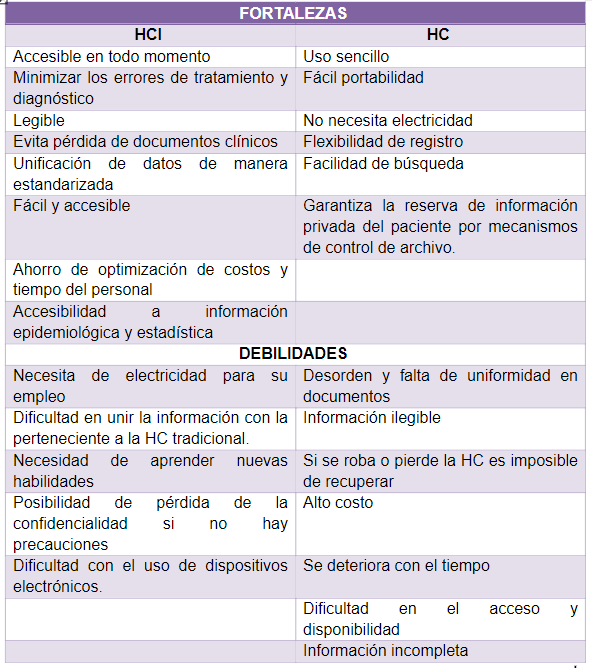
\includegraphics[]{MainMatter/HCIvsHC.PNG}
	\end{figure}
\end{center}

Los programas para el manejo de la información de la HC principalmente tienen dos componentes: una base de datos y un programa informático para suministrar y acceder a estos datos. Por el volumen de información que se maneja cada uno de estos componentes debe tener la potencia y la seguridad que garanticen un adecuado producto. Hoy son innumerables los programas y soluciones informáticas que se ofrecen en el mercado, lo cual ha generado gran cantidad de soluciones, adecuadas a los requerimientos y las exigencias de sus creadores \brackcite{rueda2006historia}. El propio autor señala que los factores que con mayor peso influyen negativamente en la adopción e implementación a nivel institucional de la HCI son:  
\begin{itemize}
	\item	Los desarrollos estandarizados (comerciales) no siempre cumplen las expectativas de los usuarios lo que genera mayor resistencia al cambio.  
	
	\item Falta de coordinación y comunicación entre los administradores y los asistenciales para la definición de la solución a implantar y el plan de trabajo para lograrlo.  
	
	\item Falta de capacitación en temas informáticos generales y específicos, a los usuarios del sistema. 
	
	\item Para unificar la terminología médica es necesario codificar el mayor número de variables posibles y este concepto no se avoca en forma anticipada, generando rechazo hacia el programa de implementación de la HCI. 
	
	\item La implementación de la HCI frecuentemente necesita cambios o rediseño de procesos administrativos y asistenciales, situación un tanto compleja de prever, y que genera un motivo adicional de rechazo.  
\end{itemize}

Ahora bien, todos los aspectos anteriormente descritos son superables mediante el desarrollo de las TIC, pero las fuentes primarias que nutren la construcción de la HCI es la actividad documentalista del equipo sanitario. Sin su participación decidida para alimentar las bases de datos en forma adecuada no se lograrían los resultados esperados, constituyen el actor primario del proceso.

\section{Estudios Previos}
\brackcite{jarrin2021diseno}
Un trabajo de vital importancia para la temática de estudio lleva por nombre \textbf{Aplicación Móvil para Centralizar Servicios de Mascotas}, elaborado por Maribel Boggio et al en el año 2017. Como objetivo central se pretende construir una aplicación móvil para centralizar servicios de mascotas. Su razón de existencia se justifica dado que en los últimos años las mascotas han ido adquiriendo mayor protagonismo en la vida de los humanos, formando parte importante del núcleo familiar y recibiendo los mismos cuidados que cualquiera de sus miembros. Las familias que tienen una mascota se preocupan cada vez más por brindarle los mejores cuidados posibles. Pero surge un inconveniente, en muchas ocasiones por más que deseen brindarles los mejores cuidados, no saben dónde es posible obtenerlos. Ignoran si los centros de asistencia a los cuales acuden tienen una buena o mala reputación, buscan servicios y muchas veces no los encuentran, desconocen ciertos tratamientos que pueden beneficiar a sus mascotas, inclusive ofertas de productos que pudieran adquirir. En términos metodológicos se realizaron varios estudios de mercado donde se evidenció una falta de servicios para las mascotas. 

Como resultado del trabajo mencionado se obtuvo la implementación de la aplicación \textbf{Guau}.
Este un proyecto factible y financieramente viable con una TIR de 29\%. Esto se sustenta en el análisis económico–financiero. El horizonte de estudio fue definido en 4 años debido a que, si bien es una solución tecnológica y todo hace indicar que continuará en ascenso, no podemos perder de vista la rapidez y evolución de este mercado. La estrategia de la empresa será de diferenciación, en el mercado no existe algo similar y el contacto con los clientes será personalizado de acuerdo a sus necesidades. Hoy en día en el Perú existe una clara preferencia por perros como mascota, por ello el desarrollo de la aplicación se centrará en canes. No debemos perder de vista al gato como mascota, el cual tiene una tendencia de crecimiento importante, aunque todavía lejos de los perros.

\brackcite{jarrin2021diseno}Otra investigación que se suma importancia para este proyecto lleva por nombre 
\textbf{Estudio para la creación de una tienda en línea para servicios veterinarios y 
productos para mascotas delimitado a Bogotá}, elaborado por Jessica Chaki 
Strelec en el año 2016, el objetivo general de este es analizar el mercado de las 
mascotas (perros y gatos) e identificar las oportunidades para la comercialización 
de productos y servicios veterinarios en línea, como metodología se tuvo la 
metodología planteada para el desarrollo de este proyecto está basada en analizar 
el objetivo del trabajo, y así, realizar consultas bibliográficas relacionadas con la 
prestación de servicios y mercadeo aplicable a una empresa veterinaria, además 
de información sobre empresas en línea. 
Al comienzo del trabajo se conseguirán datos suficientes sobre los temas 
relacionados con una empresa en-línea, productos para mascotas, mercadeo, 
servicios veterinarios; luego, se profundizará en estos temas para correlacionarlos 
y constituir una base teórica para la creación de esta empresa. Con ello, se 
realizará una investigación exploratoria, en la recopilación de información. Se 
consultarán fuentes primarias con la aplicación de encuestas para establecer la 
disposición del usuario, y secundarias, como lo son entes gubernamentales, 
universidades y portales de internet. Para la investigación exploratoria, se va a 
indagar o examinar un problema o situación para proporcionar conocimiento y 
entendimiento sobre cierto tema. Este tipo de investigación se puede utilizar para: 
formular o definir un problema con más precisión. Como resultado se obtuvo que 
este estudio está fundamentado en la propuesta que resalta la influencia de la 
21
tecnología en las nuevas generaciones y en los mercados, más específicamente, 
en el de las mascotas.

Al realizar un estudio como el que se expuso previamente, se evidenció la 
necesidad de crear lineamientos pertinentes para la creación de una página en línea. Esta irá enfocada hacia los diferentes propietarios de perros y gatos, 
principalmente desde la oferta de productos de alimentación, cuidado, salud y 
accesorios. Se genera mayor satisfacción a los clientes por el servicio prestado, 
ya que las facilidades de pago, procesos de compra, disponibilidad inmediata y el 
fácil acceso desde cualquier punto de la ciudad, por medio de cualquier dispositivo 
con conexión a internet, hace posible el llegar al consumidor y hacerle más 
sencilla la adquisición de sus necesidades.

\section{Softwares desarrollados en Cuba}
A continuación, se presentan estudios previos o antecedentes investigativos, como referentes para este proyecto, en los cuales se establecen la utilización de softwares para la prestación de servicios médicos veterinarios en Cuba. 

\subsection{Web del Registro Cubano de Mascotas (RCM)}\label{chapter:web}

%\begin{figure}[h!]
%	\begin{center}
%		
\includegraphics[scale=0.4]{Graphics/images/LogodelRegistroCubanodeMascotas.jpg}
%		\caption{Logo del Registro Cubano de Mascotas}
%		\label{fig:rcm}
%		
%	\end{center}
%\end{figure}

Luego de más de 30 años de reclamos finalmente se aprueba en Cuba un Proyecto de Ley sobre protección animal que busca defender los derechos de animales silvestres, de granja y de compañía. Los animales de granja y silvestres tienen derechos y una connotación legal y ética, pero no social. En cambio, los de compañía si pueden y deben entrar en este grupo por su vinculación estrecha al dueño, su familia y el entorno comunitario. Desde esta perspectiva se hace obligatorio que la mascota sea identificada oficialmente y cambiar su estatus de objeto a sujeto. En una reunión efectuada en marzo de 2006 en el Consejo Científico Veterinario de La Habana algunos médicos, técnicos y estudiantes veterinarios abogaron por realizar un estudio para un registro de las mascotas a través de una intranet del Instituto de Medicina Veterinaria. Su objetivo era poder acceder a los datos de las mascotas desde cualquier lugar del país.

Con este enfoque se crea la \textbf{web del Registro Cubano de Mascotas}\brackcite{insReg}, un espacio digital que brinda identificación, respaldo en el cuidado, protección y tenencia responsable de los animales de compañía. Como una de las particularidades se destaca la posibilidad de obtener un documento de identidad, totalmente gratuito, que llevará en él todos los datos de los animales que se inscriben y las de su persona responsable. Este es un proceso sencillo e intuitivo en el que se deben realizar los pasos que se enuncian a continuación:
\begin{itemize}
	\item Acceder a través del teléfono celular o una computadora al sitio www.mascotascuba.com,
	\item Completar los datos solicitados como nombre de la mascota, fecha de su nacimiento, sexo, raza, foto, dirección,
	\item Ingresar el correo electrónico o teléfono del tutor de la mascota.
\end{itemize}
Hasta agosto de 2021, estaban oficialmente registrados en la plataforma alrededor de 21 000 animales. De ellos, el $60 \%$ eran perros, $30 \%$ gatos, $7 \%$ aves y un $3 \%$ de roedores, reptiles, equinos, bovinos, porcinos, y otras especies.

\subsection{BACuba}\label{chapter:bacuba}

%\begin{figure}[h!]
%	\begin{center}
%		
\includegraphics[scale=0.09]{Graphics/images/LogodeBienestarAnimalenCuba.png}
%		\caption{Logo de Bienestar Animal en Cuba}
%		\label{fig:bac}
%		
%	\end{center}
%\end{figure}

\textbf{ BACuba} \brackcite{apMov, cubDis} es una aplicación para teléfonos móviles que tiene como fin lograr el bienestar animal y sensibilizar a las personas con la protección de estos seres. Dicha aplicación es una iniciativa de la organización \textbf{Bienestar Animal Cuba}\brackcite{pOBAC}, la mayor red de voluntarios para la protección animal. Fue lanzada desde el pasado 19 de enero de 2022, y se basa en el principio que rige la organización: rescatar animales abandonados y brindarles todos los cuidados. También buscan promover campañas, actividades, ferias y spots para garantizar el bienestar animal. Esta novedosa aplicación posee varias utilidades separadas en varias secciones:
\begin{itemize}
	\item \textbf {Adoptar}: En este panel se muestran todos los datos (nombre, edad, sexo, raza) y con una foto incluida de los animales que están en adopción, ya sea perros, gatos u otros.
	\item \textbf{Reportes}: Esta es una de las secciones más humanas, ya que los usuarios podrán reportar desapariciones de mascotas, acciones de maltrato animal, atropellos, abandonos, animales en estado de vulnerabilidad. Pueden hacerlo desde cualquier parte del país y con estas denuncias los voluntarios de las distintas redes de ayuda animal o cualquier persona sensibilizada tomará cartas en el asunto.
	\item \textbf{Cuidados}: En este apartado se brindan informaciones de mucha ayuda para los dueños de mascotas y que son útiles para todas las provincias y municipios del país. Por ejemplo, una lista con direcciones y teléfonos de las principales clínicas veterinarias, tiendas de accesorios y medicinas para sus mascotas, y algunos artículos de interés para aumentar la cultura del cuidado animal.
	\item \textbf{Noticias}: Aquí te podrás enterar de eventos relevantes como ferias de adopciones a lo largo de toda Cuba, donaciones y otras actividades en las que quizás te interese participar.
	\item \textbf{Mis Mascotas}: En este apartado podrás registrar a tus animales con sus nombres, fecha de nacimiento, y todos los datos de su carnet de identidad, en el caso de poseer uno. En esta base de datos podrás incluir, además, un registro con los días de vacunación y desparasitación, a modo de recordatorio.
\end{itemize}

Información general de BACuba:

\begin{itemize}
	\item Funciona con los datos móviles activados o por medio de servicio Wifi.
	\item Está diseñada únicamente para dispositivos móviles, con \textbf{un tamaño de 12.60 MB} y requiere una versión de Android 5.0 o versiones superiores.
	\item Es útil para cualquier lugar del país.
	\item Puede ser descargada, libre de costo, de la plataforma APKLIS.
	\item Tiene un diseño sencillo pero atractivo, y cumple con su función de informar, orientar, educar y ayudar en cuanto a materia de protección animal.
\end{itemize}

\subsection{Sistema de información para el control de expedientes clínicos para médicos veterinarios}

Sistema capaz de gestionar el control de historias clínicas veterinarias, además de la utilización con fines educativos e informativo ya que 
cuenta con las funciones de la publicación de contenidos referentes a la carrera , tales como: artículos, imágenes, foros, blog, libros, etc. Además facilita el trabajo debido a la función de guardar y exportar los reportes. \brackcite{thesisSistemaInf}

\section{Aplicaciones móviles que gestionan Historias Clínicas Veterinarias}\label{chapter:appmov}

\subsection{Dog Health}\label{chapter:doghe}

%\begin{figure}[h!]
%	\begin{center}
%		
\includegraphics[scale=0.12]{Graphics/images/LogodeDogHealth.png}
%		\caption{Logo de Dog Health}
%		\label{fig:dh}
%		
%	\end{center}
%\end{figure}


\textbf{Dog Health}\brackcite{dogHe} es una aplicación totalmente gratuita para móviles y tablets, fue creada por un comunicador italiano y solo está disponible en el idioma inglés. Creada para llevar el registro veterinario de nuestras mascotas en Android. Dentro de sus principales prestaciones se encuentran:

\begin{itemize}
	\item	Guardar los datos personales de las mascotas como su nombre, peso, fecha de nacimiento, número de chip, entre otros.
	\item	Hacer un seguimiento de anteriores visitas al veterinario.
	\item	Administrar a los veterinarios.
	\item	Hacer un seguimiento de las vacunas.
	\item	Recordatorios de citas y visitas.
	\item	Memorizar todas las administraciones de medicamentos realizadas y por realizar.
	\item Buscar y contactar con el veterinario más cercano.
	\item	Añadir múltiples mascotas.
	\item	Realizar backups y restaurarlos.
	\item	Guardar la evolución del peso y altura de las mascotas de forma continuada.
\end{itemize}


\subsection{Pet Soft}\label{chapter:petso}

\textbf{ Pet Soft}\brackcite{sofVet} \brackcite{petSo} es una plataforma para clínicas veterinarias y dueños de mascotas creada para almacenar y gestionar todo lo relacionado del paciente. Permite establecer citas, vacunas y almacenar todo tipo de información detallada con el fin de contar con un completo historial médico que le permita tanto al profesional veterinario como a los dueños de las mascotas acceder de manera segura a la información completa del animal. Esta plataforma es completamente web y la aplicación se puede descargar desde cualquier dispositivo con sistema operativo Android o IOS.

Como ventaja para el usuario, sea este médico o dueño de la mascota, la descarga de la aplicación se realiza de forma intuitiva siendo posible ingresar toda la información requerida y vital para los pacientes. Su fortaleza radica en la fácil visualización y datos de carga que aseguran una experiencia agradable para sus usuarios. Mediante el empleo de este software los usuarios pueden gestionar de forma segura y sencilla todo lo relacionado con las mascotas y acceder a la ubicación de la red más completa de veterinarias. La información de cada mascota se almacena en la web de modo que, en cada centro veterinario, se podrá descargar sin necesidad de que se tengan que volver a registrar los datos en el sistema. Dentro de sus principales beneficios para clínicas veterinarias se encuentran:

%\begin{figure}[!h]
%	\begin{center}
%		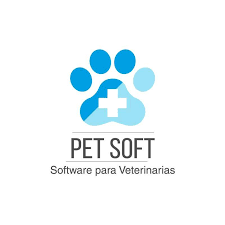
\includegraphics[scale=0.5]{Graphics/images/LogodePetSoft.png}
%		\caption{Logo de Pet Soft}
%		\label{fig:dh}
%		
%	\end{center}
%\end{figure}

\begin{itemize}
	\item	Consultas y servicios: crear consultas y servicios; todo bajo control del software,
	\item	Tarifas y bonos: manejar tus propias tarifas, generar bonos promocionales,
	\item	Citas y alarmas: notificaciones para las citas programadas o crear una directamente,
	\item	Clínicas veterinarias en red: consultar la historia clínica de la mascota si ha estado en otra veterinaria,
	\item	Médicos veterinarios: crear usuarios especializados para tu veterinaria,
\end{itemize}
Para los dueños de mascotas ofrece:
\begin{itemize}
	\item	Datos básicos: registrar todas las mascotas,
	\item	Historia clínica: llevar el historial de las consultas de tus mascotas directamente de las veterinarias,
	\item	Citas: notificaciones para las citas programadas o crear una directamente,
	\item	Veterinarias: un mapa para buscar la veterinaria más cercana,
	\item	Carné: llevar en la app el carnet de vacunación de tus mascotas.
\end{itemize}

\subsection{Petmeddata}\label{chapter:introduction}


\textbf{Petmeddata} \brackcite{petMed}\brackcite{petMed2} es un sistema electrónico seguro para almacenar el historial médico de todas las mascotas en un solo sitio. Creado en Finlandia a finales de 2018, facilita el tratamiento integral de los animales ya que muestra instrucciones de alta, medicamentos y valores de laboratorio en orden cronológico. Los problemas de seguridad se han considerado cuidadosamente. El dueño del animal decide quién puede ver la información de la mascota. Si el propietario comparte el perfil con una nueva clínica, esta puede ver las secciones más importantes del historial clínico en el historial del paciente. El personal de la clínica también ve las entradas, textos e imágenes del propietario. Nadie puede ver el precio y la información de pago, ni las notas de la clínica de animales. El nombre del animal o el microchip nunca aparecerán en ninguna parte. Para dueños de animales y clínicas de animales, el sistema es gratuito. A los socios se les cobra una tarifa por prestar sus servicios en el sistema.
“Al utilizar $Petmeddata$, el dueño siempre tiene consigo el historial médico de la mascota, incluso si va a una nueva clínica. Y el veterinario podrá leer en un formato fácil de leer lo que se le ha hecho al animal en el pasado. No hay necesidad de llevar papeles escritos a mano o impresos”, dice la Gerente de Proyecto Eva Kaisti.

Entre sus principales características se encuentran:
\begin{itemize}


\item	Fácil acceso online a todos los datos sanitarios de las mascotas; crea el perfil médico para cada uno de tus animales y contrólalos desde un solo sitio
\item	Veterinarios y otros expertos envían los datos médicos oficiales al perfil del animal.
\item	Posibilidad de añadir tus propios documentos y notas.
\item	Funciona por conexión a internet desde un teléfono móvil, tablet u ordenador.
\item	Sitio seguro; no almacena información personal tuya, sólo la información médica de tus mascotas.
\item	Posibilidad de compartir el perfil de las mascotas con un profesional del cuidado de los animales, como un veterinario, un amigo, guardería para mascotas, etc.
\end{itemize}


\subsection{VitusVet}\label{chapter:introduction}

\textbf{VitusVet} \brackcite{vitPet} es un $software$ de administración de prácticas veterinarias que permite a veterinarios y hospitales manejar el flujo de trabajo, comunicaciones con clientes, pagos, historias clínicas, horarios de consultas, entre otros. Permite el envío y recibimiento de texto, imágenes y actualizaciones en tiempo real.

Usando aplicaciones móviles de $VitusVet$ múltiples veterinarios pueden compartir historias clínicas de mascotas con clientes y hacer recordatorios sobre encuentros futuros. La plataforma $VitusPay$ permite a los dueños de mascota realizar pagos mensuales a través de tarjetas de crédito. Los clientes pueden pedir consultas con los veterinarios a través de mensajes de texto, emails, plataformas de redes sociales y aplicaciones móviles. El $software$ permite a veterinarios configurar y automatizar respuestas basándose en el personal disponible, horario de trabajo, días feriados y enviar recordatorios a través de postales personalizadas. 



\section{Conclusiones}\label{chapter:conclus}

En este capítulo se analizaron aplicaciones con similitudes a la que se plantea como finalidad en este documento. Todo esto con el objetivo de adoptar las ideas de la competencia o mejorarlas dependiendo del caso, sobre este tema se puede afirmar lo siguiente:
\begin{enumerate}
	\item	En general las herramientas en esta sección permiten la creación y el manejo de las historias clínicas digitales para nuestras mascotas, pero como se observó en cada caso estas no brindan la posibilidad para exportar de manera offline los datos de las mascotas que queramos compartir con otro usuario. Entre los objetivos de este trabajo está la mejora de este aspecto.
	\item	Pocas de estas aplicaciones permiten al usuario consultar los datos de sus mascotas sin la necesidad de una conexión a Internet, aspecto que goza de gran peso entre los principales objetivos de este trabajo.
	\item	Las herramientas para el manejo de las historias clínicas desde un dispositivo móvil, permiten a los usuarios ya sean médicos veterinarios o dueños y encargados de las mascotas acceder de manera sencilla y segura a toda la información referente al estado de salud, seguimiento, y cuidado del animal.
	\item	Luego de analizar las aplicaciones anteriores se concluye como necesario el diseño de una aplicación que cumpla con los requerimientos para el presente trabajo planteados en la introducción. En general las aplicaciones existentes no permiten el trabajo con historias clínicas animales de manera offline, aspecto de vital importancia en nuestro contexto debido a las limitaciones de la conexión a Internet que presenta nuestro país.
\end{enumerate}








